\documentclass[a4paper]{article}

\usepackage{graphicx}
\usepackage{url}

\addtolength{\textwidth}{2cm}
\addtolength{\hoffset}{-1cm}
\setlength{\parindent}{0pt}
\setlength{\parskip}{1ex}

\title{MTF Mapper}
\author{F. van den Bergh (fvdbergh@gmail.com)}

\begin{document}
\maketitle

\section{Overview}
The MTF mapper package offers a collection of tools to measure Modulation
Transfer Function (MTF) values in images. It does this by computing the edge
spread function of a step edge in an image, using the method described in
\cite{khom}.

MTF mapper offers fully automated operation, producing the following
outputs:
\begin{enumerate}
    \item Annotated images, where the MTF50 value of an edge is drawn on top
of the edge itself;
    \item Profile data sets, where the MTF50 values are represented in a
one-dimensional projection of the image. This is the tool you want if you
are interested in objectively adjusting your DSLR autofocus fine-tuning (see
Section~\ref{sec:autofocus} for details of the method).
    \item MTF surface images, where you can visualise the MTF50 values
across the focal plane, to see the image centre MTF50 relative to edge MTF50,
for example.
\end{enumerate}

MTF mapper expects images containing dark rectangular objects on light
backgrounds; the objects can be slightly out-of-square, e.g., trapezoids or
parallelograms, provided the interior angles are at least reasonably close
to 90$^\circ$.

Special test charts are required for Profile mode.
Section~\ref{sec:profile_mode} describes them in more detail.

Special test charts are also required for MTF surface mode.
Section~\ref{sec:surface_mode} describes them in more detail.

\section{Modes}
\subsection{Annotation mode (\texttt{-a} or \texttt{--annotate} flag)}
No explanation required, really. Input images are searched for rectangular
objects. Once found, the MTF50 value will be computed across each edge of
all the rectangular objects. The resulting value is drawn on top of each
edge, and the result saved as \textrm{annotated.png} by default.

\subsection{Profile mode (\texttt{-p} or \texttt{--profile} flag)}
\label{sec:profile_mode}
Using a special test chart that looks like
Figure~\ref{fig:profile_test_chart}, the program will construct a profile
such as the one shown in Figure~\ref{fig:sample_profile}, which was derived
from the original image shown downsampled in
Figure~\ref{fig:profile_test_chart_photo}. The chart should
be photographed at a $45^\circ$ angle.

\begin{figure}
\centering
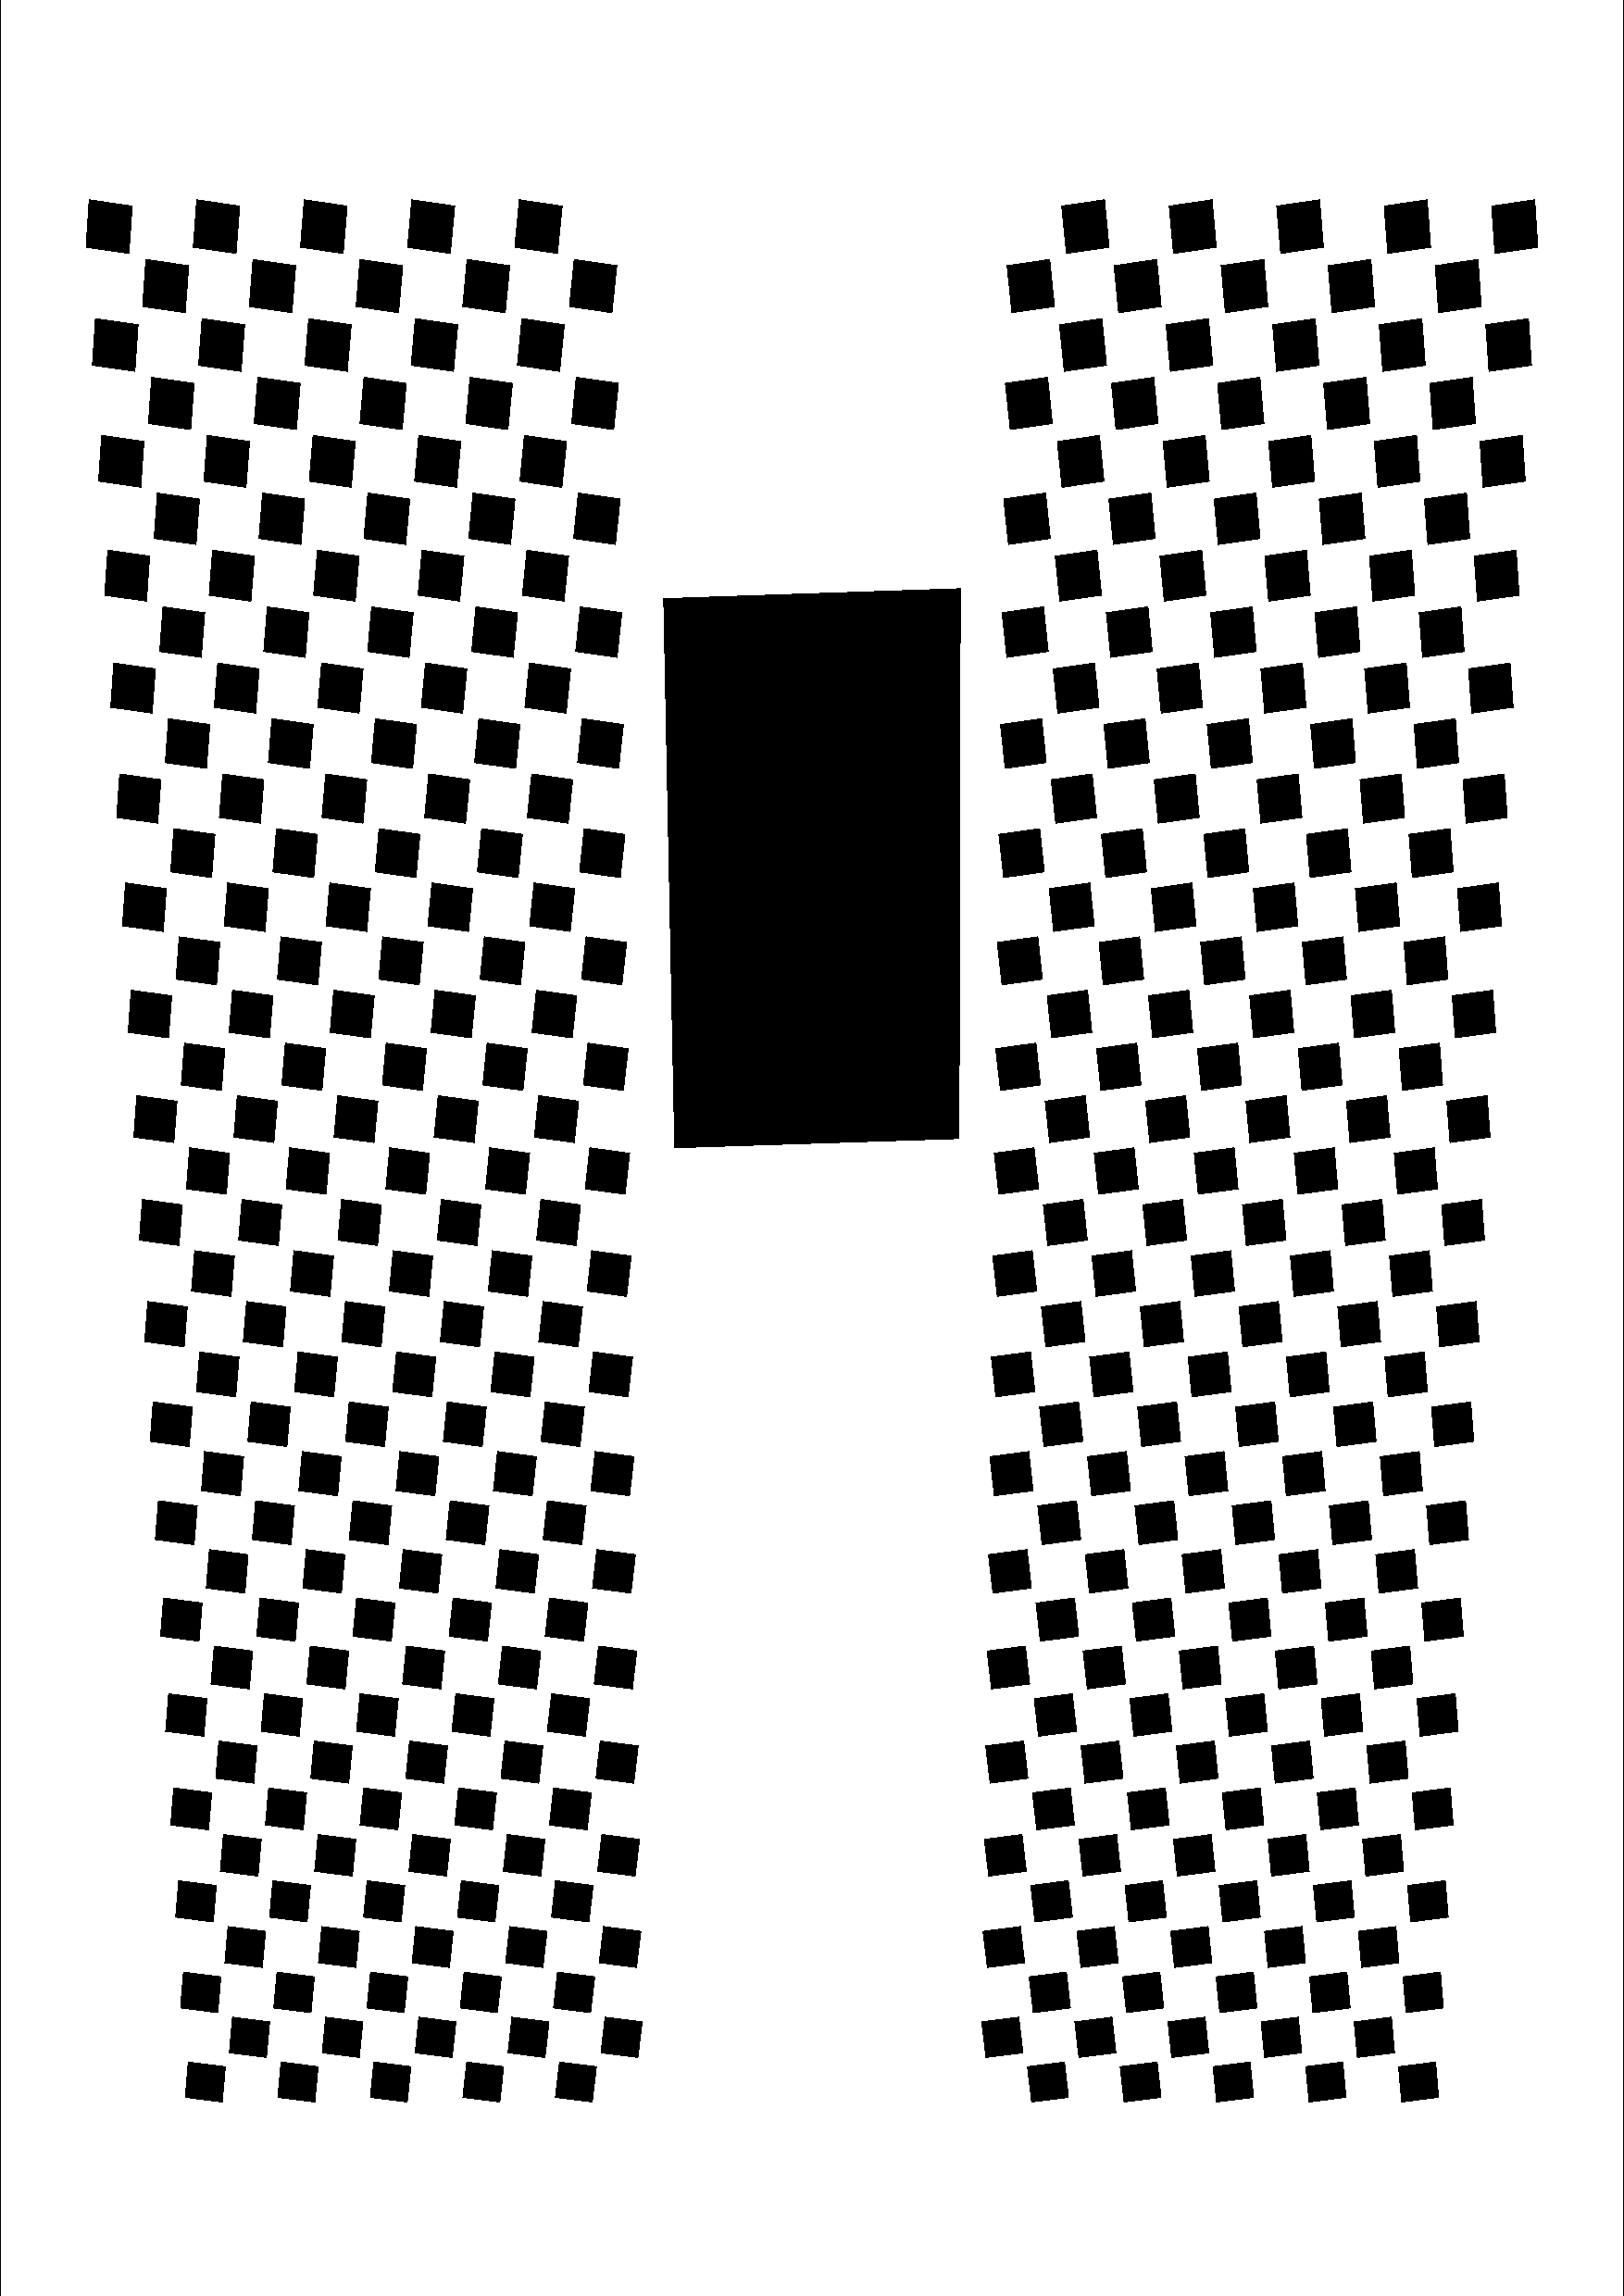
\includegraphics[width=0.4\textwidth]{figures/mtf_profile_test_chart}
\caption{Example of Profile mode test chart}
\label{fig:profile_test_chart}
\end{figure}

\begin{figure}
\centering
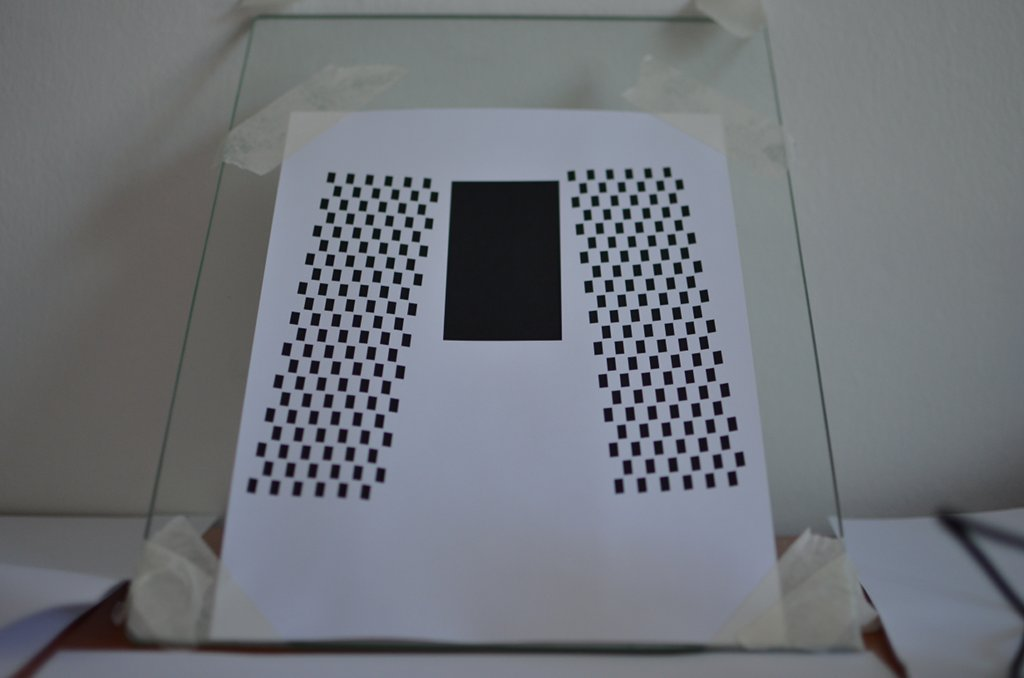
\includegraphics[width=0.4\textwidth]{figures/perspective_sample_photo}
\caption{A photo of a perspective test chart (downsampled) }
\label{fig:profile_test_chart_photo}
\end{figure}

\begin{figure}[!hb]
\centering
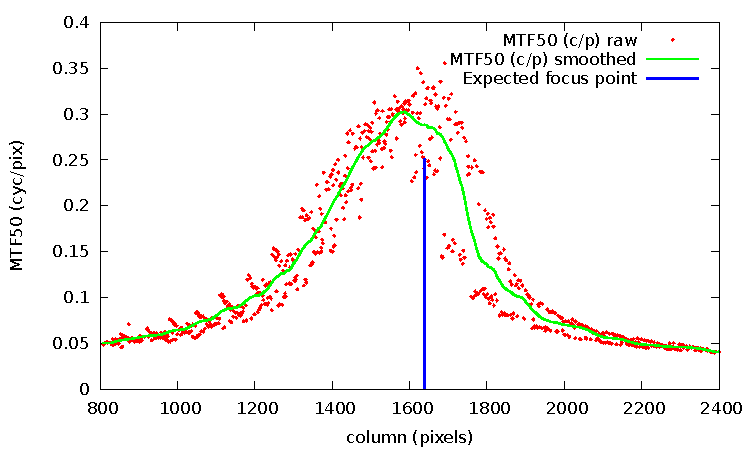
\includegraphics[width=0.95\textwidth]{figures/sample_profile}
\caption{Example of profile generated by MTF mapper. Derived from the image
shown in Figure~\ref{fig:profile_test_chart_photo}.}
\label{fig:sample_profile}
\end{figure}

The large central block is called the reference block, and the edge of this block closest to the
centroid of all blocks (the bottom edge in
Figure~\ref{fig:profile_test_chart}) is called the \emph{reference edge}.
The MTF50 values computed across the edges of all the blocks in the image
are projected onto the $y$-axis of the image, thus forming a new set of data
points of the form ($y$-value, MTF50 value). This data is seen as the red
dots in Figure~\ref{fig:sample_profile}. The \emph{reference edge} is
represented similarly, and plotted as the blue impulse in
Figure~\ref{fig:sample_profile}. A smoothed curve is constructed from the red
points, and is plotted as the green curve.

Generally, \emph{Profile} mode is only intended to be used to calibrate or
evaluate the autofocus sensor of a DSLR; the details of this process are
described in Section~\ref{sec:autofocus}.

\subsection{MTF Surface mode (\texttt{-s} or \texttt{--surface} flag)}
\label{sec:surface_mode}
%
\begin{figure}
\centering
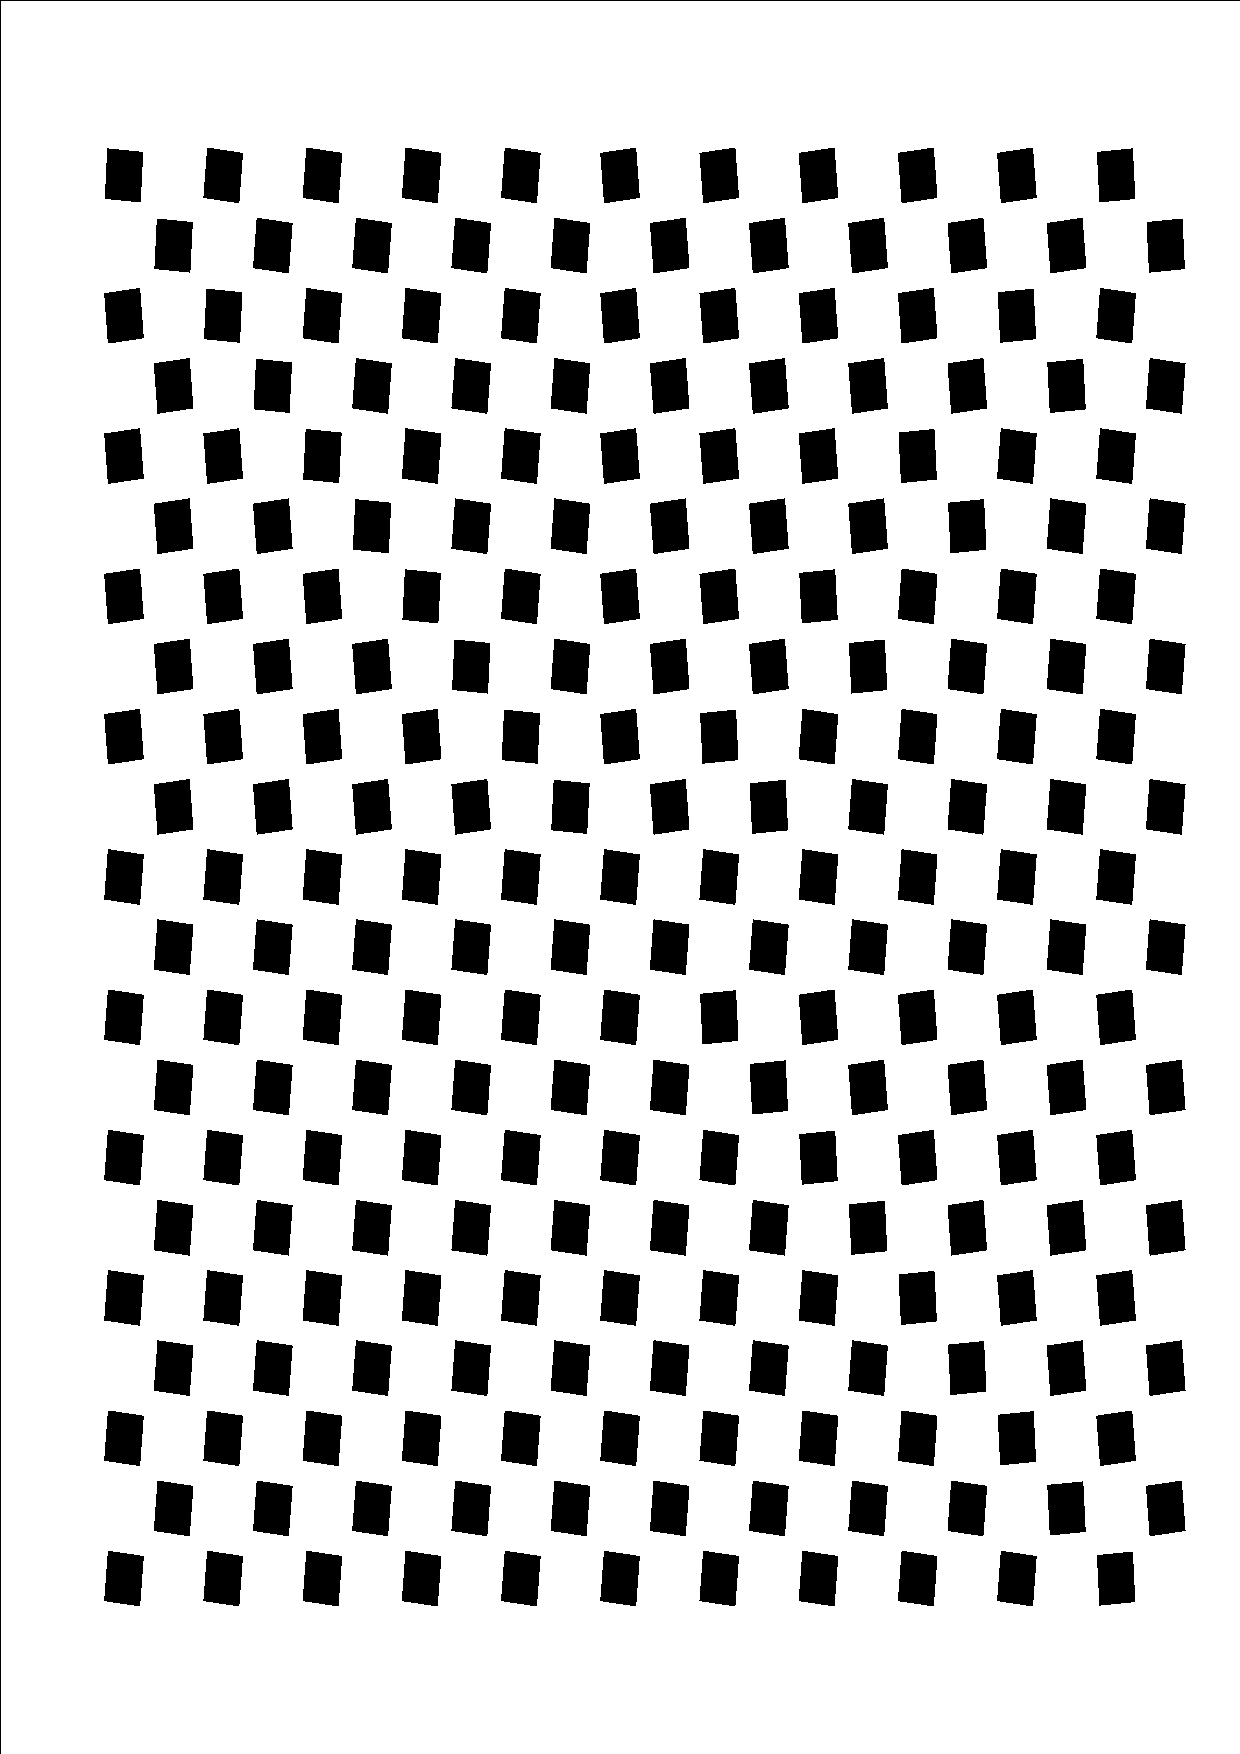
\includegraphics[width=0.5\textwidth,angle=90]{figures/mtf_surface_test_chart.pdf}
\caption{Example of an MTF surface mode test chart}
\label{fig:surface_test_chart}
\end{figure}
%
Using any test chart with a regular grid of rectangles (as illustrated in
Figure~\ref{fig:surface_test_chart}), you can measure the acuity of your
lens/camera system as it varies across the focal plane. Just shoot the chart
at a reasonable distance, making sure that it covers the entire viewfinder.
For optimal accuracy, the orientation of the blocks in the chart should be
approximately $5^\circ$ with respect to the pixel rows or columns.
The charts produced by the \texttt{generate\_test\_chart} program included
with MTF Mapper already take care of this, so you should try to capture the
chart as straight as possible. Do note that this becomes more critical at
higher sharpness settings, i.e., if you have a really sharp lens and you are
sharpening your images excessively, then you have to observe the orientation
of the chart carefully. For typical lenses and unsharpened images, 
chart alignment is not critical.

\begin{figure}
\centering
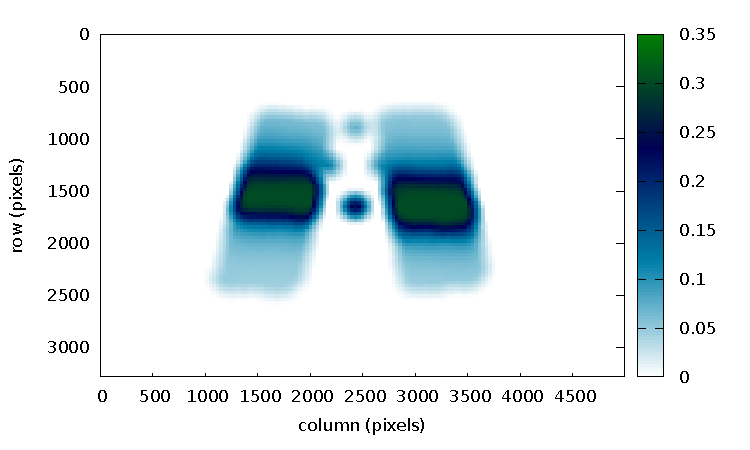
\includegraphics[width=0.95\textwidth]{figures/sample_grid_image}
\caption{Example of MTF50 image generated by MTF mapper}
\label{fig:sample_grid_image}
\end{figure}

\begin{figure}
\centering
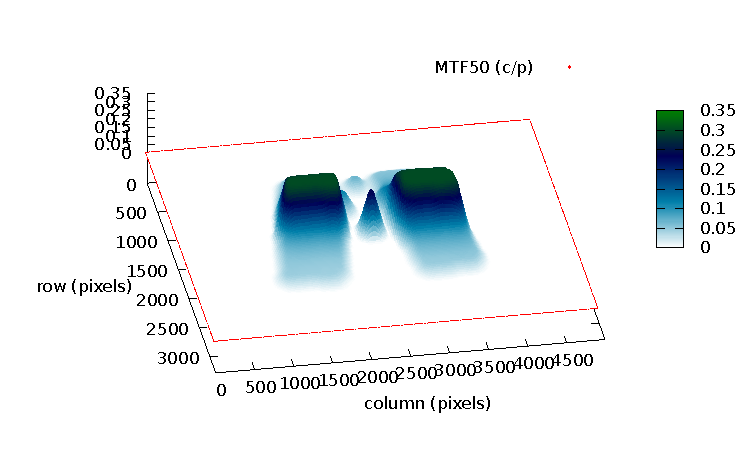
\includegraphics[width=0.95\textwidth]{figures/sample_grid_surface}
\caption{Example of MTF50 surface generated by MTF mapper}
\label{fig:sample_grid_surface}
\end{figure}

Surface mode produces two images: one representing a 2D
representation of MTF50 values across your image, and another showing the
same data as a 3D surface. Examples of both can be seen in
Figures~\ref{fig:sample_grid_image} and \ref{fig:sample_grid_surface}. These
images were obtained using a photo of the Profile mode test chart of
Figure~\ref{fig:profile_test_chart}, just because it is a bit more
interesting to look at. Since this chart was photographed at a $45^\circ$
angle, the sharpest focus is observed around the position of the reference
edge (seen as the isolated conical peak in
Figure~\ref{fig:sample_grid_surface}, and corresponding circular dot in the
centre of Figure~\ref{fig:sample_grid_image}). Focus deteriorates as you
move up or down along the image (corresponding to moving further from the
plane of focus), resulting in a decrease in MTF50 values. Incidentally, this
particular lens is now fairly close to optimally calibrated, since the
sharpest focus region is relatively well aligned with the position of the
\emph{reference edge}.


TODO: include examples of grid chart.


\section{Autofocus fine-tuning}
\label{sec:autofocus}
%
\begin{figure}
\centering
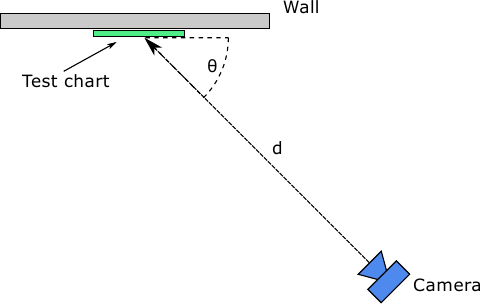
\includegraphics[width=0.95\textwidth]{figures/af_setup}
\caption{Illustration showing the top view of the autfocus calibration
set-up}
\label{fig:af_setup}
\end{figure}
%
\begin{figure}
\centering
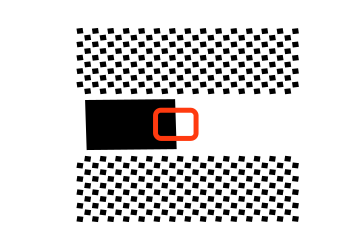
\includegraphics[width=0.95\textwidth]{figures/af_sensor_placement}
\caption{Where to place your autofocus sensor}
\label{fig:af_sensor_placement}
\end{figure}
%
The following steps can be used to calibrate the autofocus fine-tuning of a
DSLR:
\begin{enumerate}
    \item Figure~\ref{fig:af_setup} illustrates the basic set-up. The
distance $d$ is the ``distance to chart'', and the angle $\theta$ is the
``angle with respect to the test chart''.
    \item Print out the test chart at a large enough scale. Ideally, your
test chart must be large enough so that you can use it at a distance of
$30\times$ the focal length of your lens. Position your camera so that you
see the chart from an angle of at least $45^\circ$ --- the idea is that you
want some of the small blocks to be in front of the plane of focus, and some
of the blocks behind the plane of focus. The reference edge
(Section~\ref{sec:profile_mode}) should be
exactly at the plane of focus, but since you are reading this, I take it you
are still trying to adjust the autofocus fine-tuning to achieve this.
    \item Using a tripod (and remote release / timed release), take a
picture of the test chart \emph{with your chosen (centre recommended)
autofocus sensor straddling the edge of the reference block}, as illustrated
in Figure~\ref{fig:af_sensor_placement}. Take care that the autofocus sensor
is sufficiently far away from other edges (e.g., the horizontal edges of the
reference block in Figure~\ref{fig:af_sensor_placement}, or any of the small
blocks). Keep in mind that the actual sensing area of the autofocus sensor
is typically larger than the reticule you see in the viewfinder, so leave
some padding.
    \item Feed the captured image through MTF mapper to produce a profile
(such as illustrated in Figure~\ref{fig:sample_profile}. The vertical red
line denotes the position of the autofocus reference edge (at least, the one
you should have been using to focus \ldots). The green curve (or blue
points) records the MTF50 values measured along the $y$-axis of the image.
Since the test chart was at a $45^\circ$ angle with respect to the lens
axis, the $y$-axis of the image is a measure of the distance from the
camera. MTF50 values measured at different $y$-values thus indicate the
sharpness, or degree of focus, at that specific distance from the camera.
The peak of the green curve represents the plane of focus --- the objective
is to line up the peak of the green curve with the red vertical line.
    \item This procedure should now be repeated at various autofocus
fine-tuning settings on your camera. You should be able to see the peak of
the green curve shift left or right as you adjust this value. I recommend
capturing your images in batches, first stepping your autofocus fine-tuning
through the range in large steps, running the images through MTF mapper, and
then repeating this in the optimal range with smaller steps until you are
satisfied that you have calibrated your autofocus fine-tuning to the desired
level of accuracy.
\end{enumerate}

\section{Other MTF mapper utilities}
Two additional utilities are included in the MTF mapper package.
\subsection{Rectangle generator}
\label{sec:rectangle_generator}
The \texttt{generate\_rectangle} utility will create a synthetic image of a
rectangle, sampled with a specified Gaussian point spread function. The
rectangle images generated with this utility therefore have a known MTF50
value, which was calculated analytically.

In the current implementation, the Gaussian noise that is optionally added
to the image is not taken into consideration in the analytical calculation
of the expected MTF50 value. This noise certainly makes it more challenging
for software tools to compute the MTF50 values from the generated images,
but it should not bias the result in any way. 

Either way, the \texttt{generate\_rectangle} utility is useful during
testing, and can be used to cross-calibrate the \texttt{mtf\_mapper} utility
with other packages available for computing MTF50 values. (If you have
access to Imatest, please send me some results. Your feedback will help to
improve MTF Mapper).

\subsection{Test chart generator}
The \texttt{generate\_test\_chart} utility can be used to generate SVG files
containing various test charts. Currently, it can generate ``perspective''
charts that are suitable for DSLR autofocus calibration, as well as
empirical measurements of the depth of field of your equipment. It can also
generate ``grid'' charts that contain squares arranged in a regular grid,
which can be used to measure the flatness of field of your
equipment.

Currently, the MTF mapper utilities do not separate MTF50 values into
sagittal and meridional orientations, although such an option would be
relatively straightforward to add, and is planned for a future version.

\section{Frequently Asked Questions}
A bit of a misnomer, since I have yet to receive actual questions :)
\begin{enumerate}
  \item Your program gave me a value of $x$ cycles per pixel. Is this any
good? \emph{Answer}: According to Norman Koren
(\url{http://www.imatest.com/guides/modules/sfr}), a value of 0.33 cycles
per pixel is pretty good \emph{for unsharpened raw images} (emphasis mine).
This seems to roughly agree with what I see on a Nikon D7000 with the Nikkor
35 mm f/1.8 prime. Keep in mind that a Bayer colour filter sensor camera
will never be able to give you ``perfect'' MTF50 values of 0.5 c/p, and that
anything above 0.25 c/p is actually pretty good (before sharpening), 
all things considered.
  \item Cycles per pixel? I wanted lw/ph or lp/mm! \emph{Answer}: Maybe I
will add support in future versions, but you can convert manually using the
following relationship:
    \begin{eqnarray}
	\mathrm{MTF50}_{\mathrm{lp/mm}} = 
	  \frac{\mathrm{MTF50}_{\mathrm{c/p}} \times h_{\mathrm{pixels}}}{h_{\mathrm{mm}}} \\
        \mathrm{MTF50}_{\mathrm{lw/ph}} = 2 \times \mathrm{MTF50}_{\mathrm{c/p}} \times h_{\mathrm{pixels}} 
    \end{eqnarray}
where $h_{\mathrm{mm}}$ is the image height in mm, and $h_{\mathrm{pixels}}$
is the image height in pixels.
\end{enumerate}

\appendix
\section{Internal workings}
Here is a brief outline of how MTF Mapper works:
\begin{enumerate}
    \item The input image is read in, and converted to grayscale (using
OpenCV's default colour matrix). If the input image is an 8-bit image, the
pixel intensities are scaled up to 16 bits; the default is to assume that
8-bit images are sRGB gamma corrected, so the values are linearised while
begin scaled to 16 bits. If the input image has a pixel bit depth of 16
bits, no gamma conversion or scaling is applied.
    \item The image is thresholded using Bradley's adaptive thresholding 
algorithm \cite{bradley}. This is done to identify all the dark objects in
the image.
    \item The thresholded image is then scanned to extract all the connected
components using the method of Chang \textit{et al.}\cite{chang}. This step
gathers the boundary lists of all the dark objects in the image.
    \item The image gradient is computed on the original input image. This
is combined with the object boundary lists to identify all
roughly-rectangular objects (called blocks in the sequel).
    \item For each edge of each detected block, the MTF50 value is computed
as follows (roughly the method of Khom \cite{khom}):
	\begin{enumerate}
	  \item Define a rectangular buffer region that is aligned with and
centered over each edge. The width of this buffer is 32 pixels.
	  \item Compute a reasonable estimate of the orientation of the edge
(using the image gradient information).
	  \item Extract the intensity values of each pixel within the
rectangular buffer, and project the coordinates of this pixel onto the
direction normal to the edge.
          \item Systematically refine the edge normal to minimise the
difference between sequential projected values; this effectively optimises
the edge normal estimate.
	  \item For each pixel in the buffer, record a pair of values
(\textsf{distance}, \textsf{intensity}), where \textsf{distance} denotes the
length of the pixel coordinates projected onto the edge normal, and
\textsf{intensity} represents the actual pixel intensity value. Note that
the distance values are unevenly sampled. These values are a representation
of the edge spread function (ESF).
	  \item Perform LOESS fitting using a linear model to resample the 
(\textsf{distance}, \textsf{intensity}) values to a regular grid. The
resampled points are generated at a spacing of 1/32 pixels, i.e., the
profile is oversampled at a factor of 32. In addition, the derivative of the
ESF is not computed with discrete differentiation; instead, the slope of the
local linear fit is used to construct the line spread function (LSF) directly.
	  \item Apodization is performed by windowing the resampled LSF with
a Hamming window.
	  \item An FFT is computed on the resampled points, and the
normalised FFT magnitude sequence is calculated.
	  \item The frequency at which the FFT magnitude sequence reaches a
value of 0.5 is computed using linear interpolation, yielding the MTF50
value.
	\end{enumerate}
    \item The computed MTF50 values are then rendered in various ways,
depending on which output options are selected.
\end{enumerate}

\section{Accuracy}
The accuracy of the MTF50 estimates produced by MTF Mapper depends on the
following factors:
\begin{enumerate}
  \item Image resolution, and resulting edge length
  \item Image noise levels
  \item Edge orientation relative to horizontal or vertical directions
  \item Edge MTF50 value --- the sharper the edge, the more critical the
  above factors become
\end{enumerate}

\begin{figure}
\centering
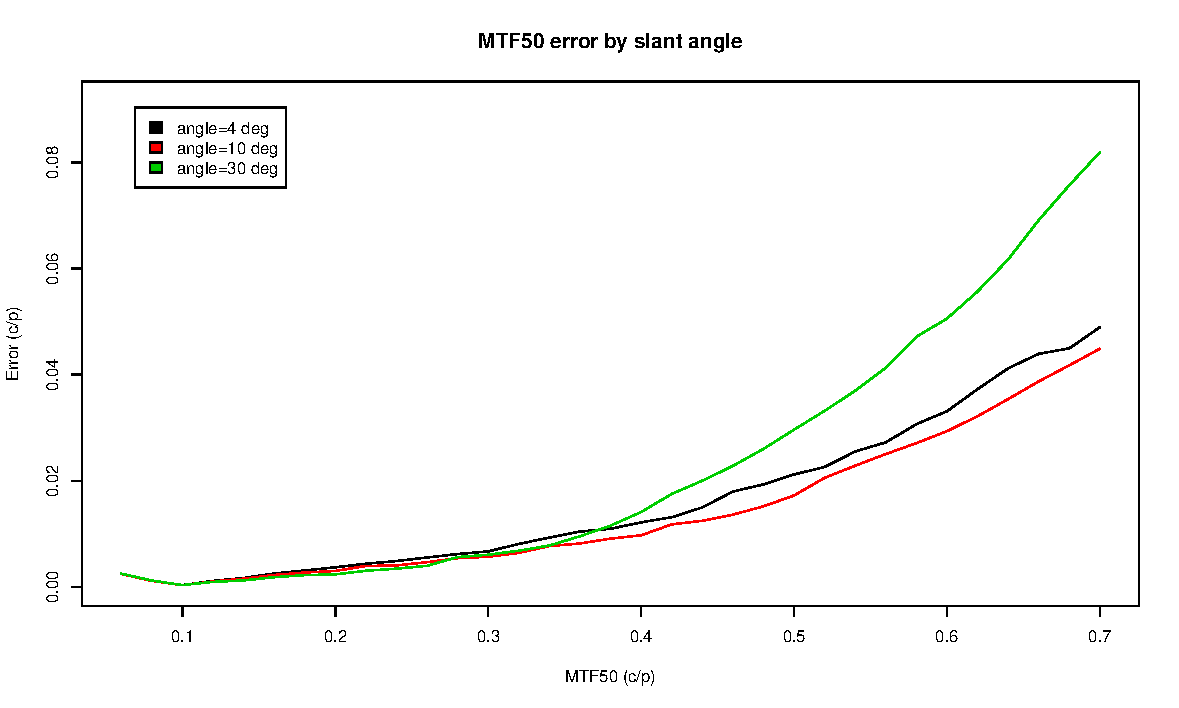
\includegraphics[width=0.95\textwidth]{figures/accuracy_plot}
\caption{Median error in MTF50 accuracy at various levels of edge acuity}
\label{fig:mtf_accuracy}
\end{figure}

Figure~\ref{fig:mtf_accuracy} presents an indication of the error in MTF50
estimates. The following parameters were fixed for this set of results:
\begin{enumerate}
  \item Resolution: an image of $300\times300$ pixels was generated using
\texttt{generate\_rectangle} (Section~\ref{sec:rectangle_generator}), 
containing a rectangle with edge lengths of $75\times100$ pixels.
  \item Noise was set to 1\% of dynamic range, \emph{before} gamma
correction to sRGB. Reverse gamma correction was applied in
\texttt{mtf\_mapper}, but some quantization error would remain.
  \item Edge MTF50 values over the range [0.06,0.7) were sampled.
  \item Edge orientations of $4^\circ$, $10^\circ$ and $30^\circ$ were
explored.
  \item A total of 30 runs (different random seeds for image noise) were
performed for each data point. Plotted values are the median over each set
of 30 values.
\end{enumerate}
The median absolute error in MTF50 estimates shown in
Figure~\ref{fig:mtf_accuracy} clearly illustrates how the error increases
with higher edge acuity, especially at slant angles that are further from
ideal. Sharp lenses should produce values in the range of (0.2,0.35) cycles
per pixel using unsharpened raw images; in this range the median error in
MTF50 estimates is below 5\%, even for slant angles of $30^\circ$.

The slight uptick in error below MTF50 values of 0.1 is most likely not an
artifact; it is probably caused by the 32-pixel window (measured normal to
the edge) that is used to compute MTF50 values. This is a trade-off: a
larger window would allow more accurate estimates down to very low MTF50
values, but would require an increase in the distance between blocks in the
image.



\begin{thebibliography}{9}
\bibitem{khom} Kohm, K., \newblock{Modulation transfer function measurement
method and results for the Orbview-3 high resolution imaging
satellite}, \newblock{Congress International Society for Photogrammetry and Remote
Sensing}, 20:12--23, 2004.
\bibitem{bradley} Bradley, D. and Roth, G.,
\newblock{Adaptive thresholding using the integral image},
\newblock{\textit{Journal of Graphics, GPU, \& Game Tools}}, \textbf{12(2)}:13--21,
2007.
\bibitem{chang} Chang, F., Chen, C.J., Lu, C.J.,
\newblock{A linear-time component-labeling algorithm using contour tracing
technique},
\newblock{\textit{Computer Vision and Image Understanding}}, \textbf{93(2)}:206--220,
2004
\end{thebibliography}

\end{document}
